\documentclass{article}
\usepackage[utf8]{inputenc}
\usepackage[T1]{fontenc}

\title{Training An Agent for Audio Source Localization}
\author{Jake Lambert \and Harris Davidson \and Rachel Ellinger}
\date{\vspace{-1em}}

\usepackage{natbib}
\usepackage{graphicx}
\usepackage{array}

\begin{document}

\maketitle

% for final report only
%\begin{abstract}
%A one paragraph high level description of the work. The abstract is typically the first thing someone would read from the paper before deciding whether to continue reading and hence, serves as an advertisement to the reader to read the whole paper. 
%\end{abstract}

\section{Introduction}

% DRAFT. Requirements (from the course template): describe the problem in a
% non-technical manner (no math or equations) and motivate it, i.e., explain
% why it is important.

When you hear a sound you cannot place, you rarely stay still. You turn your head, listening as your head turns towards the predicted location of the source, gathering information until the location of the sound source is solidified. Listening is an active process. Where you turn your head determines the cues that you hear, and what you hear determines where you should turn your head to optimize the information that is received next. This project asks whether a reinforcement learning agent can learn to do that same skill.

This experiment proposes a simplified version of the problem of audio source localization, also known as sound localization. There is a "head", which can be represented in programming simulation or in hardware as two microphones sitting on a motorized "head" that can turn left and right, and somewhere in the room is a sound source, which may be static or dynamic. The agent's job is to identify where the sound is coming from as accurately and quickly as possible. Keeping the head still is often not enough to locate a sound. With only two microphones, similar to having only two ears, there is cone of confusion where different sound sources have identical interaural time (ITD) and level (ILD) difference cues. Because the sound cues are identical, this creates the brain has trouble identifying where the sound is coming from, confusing between hemifield sound sources such as front/back horizontally or above/below vertically. For example, the sound from 0 degrees azimuth and 180 degrees azimuth essentially provide identical sound cues, so a stationary listener cannot reliably tell the location of the sound source \cite{kapralos2008virtualaudiosystems}. Turning the head, and thus creating dynamic ITD and ILD sound cues associated with head rotation helps listeners to resolve ambiguities in sound localization \cite{Wallach1940headmovement}. However, when considering this phenomenon, every turn costs time and energy, and in real life applications, a moving sound source will not wait for the agent. Therefore the agent faces a planning problem where it has to decide how to turn so that it maximizes collection of information to locate the sound source without wasting effort on movements that provide minimal information and know when it has heard enough to commit to an answer.

\begin{figure}[htbp]
  \centering
  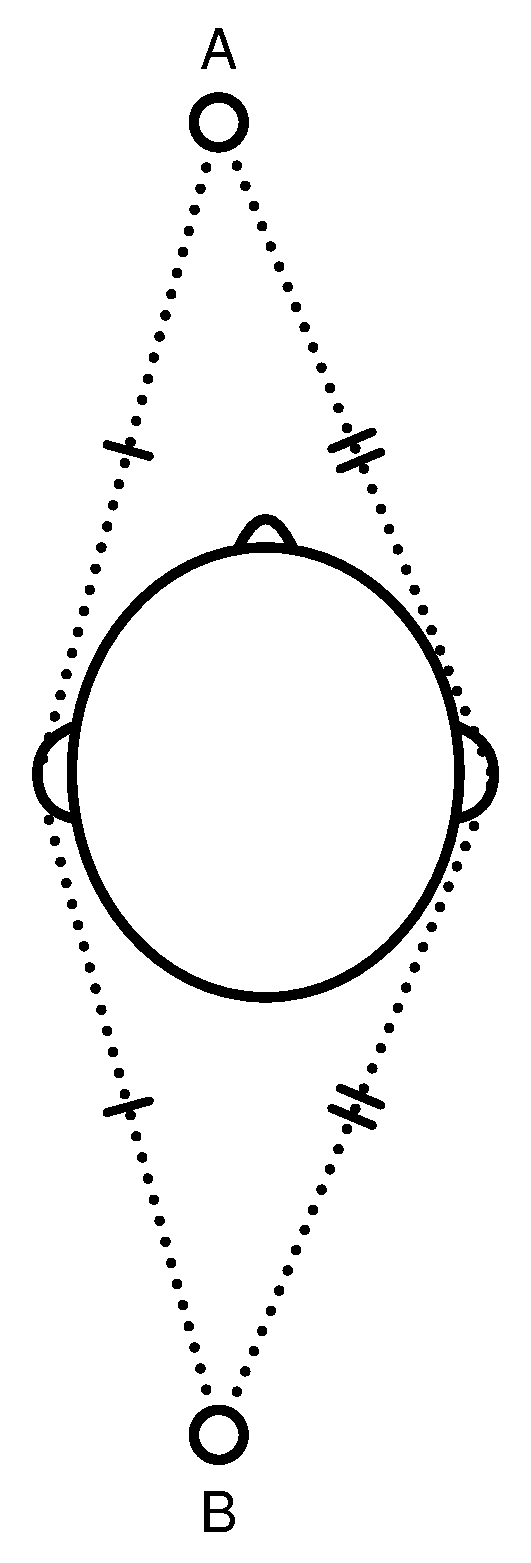
\includegraphics[height=0.35\textheight,keepaspectratio]{images/front-back-ambiguity.pdf}
  \caption{Sounds from points A and B are not distinguishable to a static head with binaural hearing in an idealized, anechoic room.}
  \label{fig:front-back-ambiguity}
\end{figure}

This makes the task a natural fit for reinforcement learning. Rather than hand-coding a search strategy, we let the agent learn through trial and error, rewarding it for labeling the correct source direction (within a fixed tolerance)
and penalizing it for every turn it takes and every wrong guess. We then compare what it learns against simple strategies, such as turning at random or following a fixed routine that turns until the sound is centered and then checks against corresponding points on the cone of confusion where ITD values are shared.

First we train the agent in a simulated room, which allows for control of exactly what it hears and the ability to run more trials than would be practical with real equipment. We start with the simplest version of the problem, a quiet room with no reverberation and a single stationary source playing white noise and train the agent across multiple reinforcement learning algorithms. Then as a second goal to determine if a policy can transfer to new conditions, we can then add elements one step at a time, such as echoes, competing sounds, small imperfections like noise from the microphones and motor, a dynamic audio source, or a second direction of rotation. We also aim as a third stretch goal to build a small physical head with a pair of microphones on a motor to test whether behavior learned in simulation holds up in a real room and to demonstrate the result in order to determine if the learned strategy transfers to a robot.

The problem matters well beyond this setup. Robots that work alongside people need to turn toward someone who speaks to them, search-and-rescue systems may need to find a person through their call for help, and devices such as smart speakers, security cameras, and hearing aids all benefit from having information about where a sound is coming from. In each case, sensors are limited and time matters, so the ability to choose where to "listen" next is integral. Additionally, the common principles of head movement patterns for sound localization in humans are poorly understood and an active area of research. Better understanding these patterns would help inform treatment for patients with hearing impairments. RL agents provide an alternative vector to study the theory of learned sound localization at a lower cost compared to human studies. 

\section{Background Related Work}

Audio source localization is a popular topic of research across both hearing sciences and machine learning, and more recently has seen conceptual integration across the two fields. Here, we propose extending this task to reinforcement learning for sound localization, a less researched area of study, as seems only natural considering reinforcement learning's strengths in sequential decision making towards optimizing the achievement of a goal state under uncertainty.

\subsection{Auditory cues and localization}
To perform the task of auditory localization, the brain requires the primary information obtained from timing, intensity, and frequency of the perceived sound ITDs, ILDs, and Head Related Transfer Function (HRTF), as well as secondary information such as relative motion and reverberation \cite{carlini2024audiolocalizationsummary}.

\subsection{Computational sound source localization}

Classical methods in engineering treat localization as a signal-processing problem where factors such as time differences of arrival between microphones and direction of arrival, as obtained through methods like beamforming, are combined through triangulation or multilateration with Gaussian mixture models to create propogation models for localization \cite{jekaterynczuk2023survey}. Meanwhile, more recent machine learning-based methods have replaced hand-selected feature computations with networks trained on simulated or recorded data, including convolutional neural networks, convolutional-recurrent networks, residual networks, and transformers \cite{jekaterynczuk2023survey, grumiaux2022survey}. Deep neural networks trained on binaural audio in simulated reverberant environments can also be used to reproduce features of human localization behavior \cite{francl2022deep}. Work by Ma et al. (2017) has found that, similar to established hearing sciences research, the addition of head rotation information in a deep neural network model resolves front-back confusion by allowing models to access ILDs and generate a more accurate cross-correlation function in addition to already available ITD cues \cite{ma2017exploiting}. Across the literature, however, the listener is almost always passive, whereby the network maps a fixed recording to a location estimate and has no control over what is heard next.

\subsection{Active-localization and machine hearing in robot audition}

A small subset of research in robot audition has explored sensor movement for localization and found that treatment of head motion as an estimation-and-control problem has allowed a robot to improve localization performance. One such study used active exploration in the horizontal plane to assess sound source azimuth and distance estimates via a Monte Carlo framework integrating probabilistic modeling using particle filtering \cite{schymura2017monte}, while a separate study focused on Monte Carlo tree search method to achieve similar long-term planning \cite{Nguyen2017mcts}. Short-term, one-step-ahead calculations have also been applied to greedily select the best movement that will provide the most new information about where a sound is originating \cite{bustamante2016one}. While these methods show that motion improves localization, their motion policies are manually designed and require online search, which is expensive and must be re-established whenever the sensing model changes.

\subsection{Reinforcement learning for auditory agents}

Reinforcement learning has been applied to auditory agents mainly in embodied
navigation. In audio-visual navigation, an agent moves through a simulated 3D
environment toward a sound-emitting target using egocentric vision and binaural
audio \cite{chen2020soundspaces}. Later work extended this to moving sound sources and distractor sounds \cite{younes2023catch} and to moving in order to hear a target more clearly \cite{majumder2021move2hear}.

Closest to our project, Ledder et al. (\cite{ledder2025audio}) trained an agent using a deep Q-learning framework to orient a head towards a talker from stereo speech recording alone. The authors found that the agent trained in medium to high reverberant environments displayed greater generalization across a range of naturalistic acoustic environments. These studies establish that reinforcement learning agents can exploit traditional sound localization ITD and ILD cues, as well as spatial audio through head movements and information derived from reverberation.

\subsection{Gap and Contribution}

Prior active-localization systems rely on manually-designed or search-based motion strategies, while reinforcement learning work on auditory agents has focused on navigation and orientation rather than on the information-gathering decision itself. To our knowledge, no work has trained a reinforcement learning agent to decide when and how to turn a two-microphone head specifically to resolve front-back ambiguity, nor compared against learned policies achieved from multiple different algorithms versus classical head-turn strategies. Our project thus attempts to address this gap.










% Following, you should provide the necessary background and discuss related work in the RL literature. This section should also be about a page. Citations should be in BibTeX format \citep{thrun2005probabilistic}. Some approaches have proposed using RL for robot soccer \cite{riedmiller2009reinforcement}.

\section{Technical Approach / Methodology / Theoretical Framework}

% for proposal
Describe how you will approach the problem and its technical formulation. Feel free to re-state the basic RL formulas (e.g., if using Q-learning, state the update rule or the formula for what the Q function approximates). 


% for final report
%A detailed description of your problem (with math, notation, algorithms, figures, etc.). Use footnotes to cite links to your code or videos\footnote{All developed source code for this project is available at ...}

\subsection{Tasks}
\label{sec:tasks}

We break the project into six areas of work. Each builds on the ones before it,
and we plan to get the simplest version of the full pipeline (environment,
agent, harness, one experiment) working before adding complications.

\begin{enumerate}
  \item \textbf{Simulation environment.} A simulated room in which a
  two-microphone head turns left and right and listens to a sound source.
  \begin{enumerate}
    \item Hidden state (never observed by the agent): the true azimuth of the sound source ${\theta}$, and the current head angle ${\hat\theta}$.
    \item Observation (the agent's input): interaural time difference (ITD) precalculated by pryoomacoustics, an acoustics python package, for each head angle and source azimuth. Noise is added as $\varepsilon_t \sim \mathcal{N}(0, \sigma^2)$ for each sample, where $\sigma$ is an experimental parameter. For agents that can only use discrete observations, the ITD is bucketed into 5 bins: far left, left, center, right, and far right.
    \item Actions: turn left, turn right, listen, stop and declare the direction. Turns move $\pi / 20 \approx 9^\circ$ which corresponds to 5 steps of NEMA 17 stepper motors. 
    \item Rewards: $-1$ per step, $$r = 100\left(1 - \frac{\Delta\theta}{\pi}\right)$$ where $\Delta\theta = \arccos\bigl(\cos(\theta - \hat{\theta})\bigr) \in [0, \pi]$ is the angle between the true and guessed directions, measured the short way around the circle.
    \item Episode termination: when the agent declares the direction or after a maximum number of steps.
    \item Configurable complications, added one at a time: echoes, noise, and a second axis of rotation.
  \end{enumerate}


  \item \textbf{Agents.} Learning agents and baselines that share one
  interface, following Sutton and Barto~\cite{sutton1998reinforcement}.
  \begin{enumerate}
    \item Baselines: a random policy, and a hand-written strategy (turn until
    the sound is centered, check front against back, then declare).
    \item Tabular Q-learning and SARSA.
    \item Semi-gradient SARSA with tile coding.
    \item REINFORCE with a baseline, or actor-critic.
    \item Stretch: DQN.
  \end{enumerate}

  \item \textbf{Test harness.} Shared tooling that runs any agent in any
  environment configuration and records the results.
  \begin{enumerate}
    \item Episode runner with fixed random seeds and configurable environment
    and agent settings.
    \item Metrics: fraction of correct declarations, angular error, steps
    taken before declaring, and return.
    \item Logging, learning curves, and summary plots, saved per experiment so
    figures can be regenerated for the report.
  \end{enumerate}

  \item \textbf{Experiments.} Each experiment is a configuration of the
  harness.
  \begin{enumerate}
    \item Algorithm comparison in the base environment, against both
    baselines.
    \item Robustness to echoes and competing sounds.
    \item Robustness to microphone and motor errors.
    \item Tracking a moving source.
    \item Stretch: transfer, i.e., training in one condition and testing in
    another, including from simulation to the physical heads.
    \item Stretch: a multi-agent version modeled on the game Marco Polo.
  \end{enumerate}

  \item \textbf{Physical heads (optional).} Three two-microphone heads on
  stepper motors, used for evaluation and the demo.
  \begin{enumerate}
    \item Order parts (by Nov 9, to arrive by Nov 18).
    \item Assemble the heads and write firmware for audio capture and motor
    control.
    \item Connect the heads to the agent running on a laptop.
    \item Evaluate trained agents in a real room and record the demo.
  \end{enumerate}

  \item \textbf{Writeup.}
  \begin{enumerate}
    \item Proposal (this document).
    \item Final report: abstract; introduction (carried over from the
    proposal); background and related work; technical approach, notation, and
    problem formulation; experimental results and figures; conclusion and
    future work.
    \item Links to code and the demo video, proofreading, and submission.
  \end{enumerate}
\end{enumerate}

% for final report
%\section{Experimental Results / Technical Demonstration}

%A description of how you evaluated or demonstrated your solution.\footnote{a video of the robot doing x y z is available at...} 

% for proposal
\section{Evaluation}

\subsection{Environment}

All experiments run in our own simulated environment, built on
pyroomacoustics and specified in Section~\ref{sec:tasks}. A two-microphone
head turns in $9^\circ$ steps, so it can face 40 directions, and a stationary
source sits at an azimuth the agent never observes. On each step the agent
receives a noisy time difference between the microphones and chooses to turn
left, turn right, listen again, or stop and declare that the source is in the
direction it is facing. Each step costs $-1$, and a declaration earns
$100\,(1 - \Delta\theta/\pi)$, where $\Delta\theta$ is the angle between the
facing direction and the source. Each episode starts with the head direction
and the source azimuth drawn uniformly at random. The base condition has no
echoes and no observation noise ($\sigma = 0$). Later conditions raise
$\sigma$ and add echoes.

\subsection{Metrics}

We evaluate each trained agent with its greedy policy and exploration turned
off, on a fixed set of 1{,}000 evaluation episodes per condition. The set is
generated once from fixed random seeds, so every agent and baseline faces the
same starting configurations and the same noise. We report three primary
measures.

\begin{enumerate}
  \item \textbf{Completion rate.} The fraction of evaluation episodes in which
  the agent declares with the source within one turn of the direction it is
  facing ($\Delta\theta \le \pi/20$). Declarations outside this tolerance and
  episodes cut off at the step limit both count as failures.
  \item \textbf{Learning curve.} Average return per episode against the number
  of training episodes, averaged over at least 10 random seeds with the spread
  across seeds shown. We use it to judge whether and how quickly each
  algorithm converges.
  \item \textbf{Fraction of optimal return.} The agent's average return
  divided by the average return of an oracle that knows where the source is,
  plotted over training alongside the learning curve. The oracle turns the
  short way round to the direction nearest the source and declares. A $9^\circ$
  turn costs 1 and raises the declaration reward by 5, so turning all the way
  is always worthwhile. From a start that is $d$ turns from that direction,
  the oracle's return is
  \begin{equation}
    G^{*} = 100\left(1 - \frac{\Delta\theta_{\min}}{\pi}\right) - (d + 1),
  \end{equation}
  where $\Delta\theta_{\min} \le \pi/40$ is the error that remains at the
  nearest direction. Averaged over uniformly random starts, $G^{*}$ is about
  88. The oracle skips the turning and listening that a real agent needs in
  order to find the source, so 100\% is an upper bound rather than a target.
  At the other end, an agent that declares at once without turning earns 49
  on average, about 56\% of the oracle's return, so values near that level
  indicate that nothing has been learned.
\end{enumerate}

As secondary measures we report the angular error at the declaration, the
number of steps taken before declaring, and how many of those steps are
spent listening rather than turning.

\subsection{Success Criteria}

In the base condition, we consider an agent successful if it completes at
least 99\% of the evaluation episodes, its learning curve levels off across
seeds, and it reaches at least 90\% of the oracle's return. We will run the
hand-written strategy first to confirm that these thresholds are attainable
with the observations the agent receives; if that strategy falls short of
them, we will say so and judge the agents against it instead. For the project
as a whole, success means that at least the tabular agents meet these criteria
and that we can compare all agents against both baselines in the harder
conditions. In those conditions no fixed threshold is meaningful in advance,
because noise and echoes may make some episodes impossible to solve, so we
report each agent's completion rate and return relative to the hand-written
strategy under the same condition. If the physical heads are built, we will
also run the trained agents on them in a real room as a check on the
simulated results, without a pass threshold.

\subsection{Hypotheses}

\begin{enumerate}
  \item In the base condition, every learning agent meets the success criteria
  and matches the hand-written strategy's return.
  \item The agents learn the front-back check without being told about it:
  when the sound starts out centered, the learned policy turns before it
  declares.
  \item As observation noise increases, the learned agents listen more often
  before they turn or declare, and they lose less completion rate and return
  than the hand-written strategy, whose rule does not change with the noise
  level.
\end{enumerate}

% for final report
%\section{Conclusion and Future Work}

%A high level summary of what was accomplished, along with a discussion on limitations and avenues for future work (typically 2 to 3 paragraphs). 


\section{Timeline and Individual Responsibilities}

The proposal is due Friday, November 13 at 11:40\,pm, and the final report is
due Wednesday, December 23 at 5:00\,pm. Table~\ref{tab:timeline} lays out the
weeks in between, with the milestones we want to reach by the end of each
week. The week of November 23 includes Thanksgiving, so it carries less work.
Weeks 6 and 7 leave room to absorb slippage before the deadline; stretch goals
are pursued only if the core experiments are done.

Table~\ref{tab:responsibilities} lists who is responsible for each area of
work. Owners have not been assigned yet and are marked TBD; we expect
assignments to shift as the project progresses.

\begin{table}[!htbp]
\centering
\small
\begin{tabular}{|l|>{\raggedright\arraybackslash}p{0.85in}|>{\raggedright\arraybackslash}p{2.3in}|p{0.45in}|}
\hline
\textbf{Week} & \textbf{Dates} & \textbf{Milestones} & \textbf{Owner} \\
\hline
1 & Nov 9--15 &
Proposal submitted (Nov 13). Base simulated room running with precomputed
responses. Physical parts ordered (optional). & TBD \\
\hline
2 & Nov 16--22 &
Environment interface complete. Random and hand-written baselines run end to
end through the test harness, with metrics and plots. & TBD \\
\hline
3 & Nov 23--29 &
Tabular Q-learning and SARSA trained in the base environment
(Thanksgiving week). & TBD \\
\hline
4 & Nov 30--Dec 6 &
Tile-coding SARSA and a policy-gradient agent working. Algorithm comparison
experiment complete. Echoes, competing sounds, and sensor errors added to the
environment. Physical heads assembled (optional). & TBD \\
\hline
5 & Dec 7--13 &
Robustness and moving-source experiments complete. Real-room evaluation
(optional). Introduction and background for the final report drafted. & TBD \\
\hline
6 & Dec 14--20 &
Stretch goals if ahead. Full draft of the final report by Dec 18. Demo video
recorded. & TBD \\
\hline
7 & Dec 21--23 &
Revisions and proofreading. Final report submitted (Dec 23, 5:00\,pm). & TBD \\
\hline
\end{tabular}
\caption{Weekly timeline and milestones.}
\label{tab:timeline}
\end{table}

\begin{table}[!htbp]
\centering
\small
\begin{tabular}{|>{\raggedright\arraybackslash}p{1.2in}|>{\raggedright\arraybackslash}p{2.4in}|p{0.45in}|}
\hline
\textbf{Area} & \textbf{Task} & \textbf{Owner} \\
\hline
Environment & Base room and precomputed responses & TBD \\
 & Observation model and environment interface & TBD \\
 & Complications (echoes, competing sounds, errors, moving source, second axis) & TBD \\
\hline
Agents & Random and hand-written baselines & TBD \\
 & Tabular Q-learning and SARSA & TBD \\
 & Semi-gradient SARSA with tile coding & TBD \\
 & REINFORCE / actor-critic & TBD \\
 & DQN (stretch) & TBD \\
\hline
Test harness & Episode runner and configuration & TBD \\
 & Metrics, logging, and plots & TBD \\
\hline
Experiments & Algorithm comparison & TBD \\
 & Echoes and competing sounds & TBD \\
 & Microphone and motor errors & TBD \\
 & Moving source & TBD \\
 & Transfer and sim-to-real (stretch) & TBD \\
 & Marco Polo (stretch) & TBD \\
\hline
Hardware (optional) & Parts, assembly, and firmware & TBD \\
 & Real-room evaluation and demo & TBD \\
\hline
Writeup & Proposal & TBD \\
 & Literature review and related work & TBD \\
 & Technical approach and notation & TBD \\
 & Results and figures & TBD \\
 & Abstract, conclusion, and final editing & TBD \\
\hline
\end{tabular}
\caption{Individual responsibilities.}
\label{tab:responsibilities}
\end{table}

%\cite{short2010no}.

% Print any pending tables before the references.
\clearpage

\bibliographystyle{plain}
\bibliography{references}
\end{document}
